%!TEX output_directory = temp
\documentclass{amsart}
	%% boilerplate packages
		\usepackage{amsmath}
		\usepackage{amssymb}
		\usepackage{amsthm}
		\usepackage{enumerate}
		\usepackage{mathrsfs}
	%% graphics stuff
		\usepackage{graphicx}
		\graphicspath{{../images/}}
	%% my shorthand
		\DeclareMathOperator{\SE}{\text{SE}}
		\DeclareMathOperator{\Paup}{\text{Paup}}
		\DeclareMathOperator{\Out}{\text{Out}}
		\DeclareMathOperator{\Old}{\text{Old}}
		\DeclareMathOperator{\Pop}{\text{Pop}}
		\DeclareMathOperator{\Ell}{\mathscr{L}}
	%% Levin's shorthand
		\newcommand{\E}{{\mathcal{E}}}
		\newcommand{\A}{{\mathcal{A}}}
		\newcommand{\B}{{\mathcal{B}}}
		\newcommand{\R}{{\mathbb{R}}}
		\newcommand{\X}{{\mathbf{X}}}
		\newcommand{\x}{{\mathbf{x}}}
		\newcommand{\M}{{\mathcal{M}}}
		\newcommand{\var}{{\rm Var}}
		\newcommand{\ep}{\varepsilon}
		\newcommand{\sd}{{\rm SD}}
		\newcommand{\bvec}[1]{{\boldsymbol #1}}
		\newcommand{\bbeta}{\bvec{\beta}}
		\newcommand{\bX}{\bvec{X}}
		\newcommand{\ssreg}{{\rm SS}_{{\rm Reg}}}
		\newcommand{\ssr}{{\rm SS}_{{\rm Res}}}
		\newcommand{\sst}{{\rm SS}_{{\rm Tot}}}
	%% Homework details
		\usepackage{hyperref}
		\usepackage{color}
		\renewcommand{\abstractname}{Introduction}
		\author{Alex Thies}
		\title{Homework 2 \\ Math 463 - Spring 2017}
\begin{document}
	\begin{abstract}
		I collaborated with Joel Bazzle, Torin Brown, Ashley Ordway, and Seth Temple on this assignment. 
		The histograms, and scatter plots which are requested in Problems 1 and 2 are bunched together at the end of assignment; trying to make them appear in a neat manner throughout the document proved difficult.
	\end{abstract}

	\maketitle

	\section{A regression model} % (fold)
	\label{sec:a_regression_model}
		\subsection{Assingment} % (fold)
		\label{sub:assingment1}
			In this part, you will replicate Yule's regression equation for the metroplis unions, 1871-81. 
			See Chapter 1 of Freedman (2009) for a discussion. 
			Fix the design matrix $\X$ at the values reported in Table 3 there, available at 

			\color{red}\url{http://pages.uoregon.edu/dlevin/DATA/yule.txt}
			
			\color{black}(Subtract 100 from each entry to get the percent changes.) 
			Yule assumed $$\Delta \Paup_{i} = a + b \cdot \Delta \Out_{i} + c \cdot \Delta \Old_{i} + d \cdot \Delta \Pop_{i} + \ep_{i}$$ for 32 mentropolitan unions $i$. 
			For now, suppose the errors $\ep_{i}$ are I.I.D., with mean 0 and variance $\sigma^{2}$.
			\begin{enumerate}[(a)]
				\item Estimate $a$, $b$, $c$, $d$ and $\sigma^{2}$.
				\item Compute the $\SE$’s.
				\item Are these $\SE$s exact, or approximate?
				\item Plot the residuals against the fitted values. 
				(This is often a useful diagnostic: If you see a pattern, something is wrong with the model.
				You can also plot residuals against other variables, or time, or \dots)
			\end{enumerate}
		% subsection assingment (end)

		\subsection{Solution} % (fold)
		\label{sub:solution1}
			We estimate the coefficients, standard deviation, standard errors, and residuals of Yule's linear model with R.
			In Figure \ref{lmsummary}, we have the summary of the linear model, showing the values of the estimates and standard errors for the coefficients $a$, $b$, $c$, and $d$.
			\begin{figure}[b]
				\begin{tabular}{ccccc}
					\hline 
					Coefficients & Estimate & $\SE$ & $t$ value & Pr$(>|t|)$ \\
					\hline
					\hline
					a & 12.88356 & 10.36722 & 1.243 & 0.224 \\
					b & 0.75209 & 0.13499 & 5.572 & 5.83e-06 *** \\
					c & 0.05560 & 0.22336 & 0.249 & 0.805 \\
					d & -0.31074 & 0.06685 & -4.648 & 7.25e-05 *** \\
					\hline
				\end{tabular}

				Residual standard error: 9.547 on 28 degrees of freedom.

				Multiple R-squared: 0.6972, Adjusted R-squared: 0.6647.

				F-statistic: 21.49 on 3 and 28 DF, $p$-value: 2.001e-07
				\caption{Summary of Linear Model}
				\label{lmsummary}
			\end{figure}
			Note that the standard errors are approximations because they are constructed from the estimated coefficients, which are themselves approximations. 
			Furthermore, from the summary we see that the residual standard error is $\sigma = 9.547$, thus $\sigma^{2} = 91.1452$.
			Figure \ref{scatterplot1} is the plot of residuals, $e_{i}$, against the fitted values $\hat{y}_{i}$. 
			There is no discernible pattern, the points appear to have low correlation.

		% subsection solution (end)
	% section a_regression_model (end)

	\section{The \textit{t}-Test} % (fold)
	\label{sec:the_t-Test}
		\subsection{Assignment} % (fold)
		\label{sub:assignment2}
			Make a $t$-test of the null hypothesis that $b = 0$. 
			What do you conclude? 
			If you were arguing with Yule, would you want to take the position that $b = 0$ and he was fooled by chance variation?
			In this part, you will do a simulation to investigate the distribution of $t = \hat{b}/\SE$, under the null hypothesis that $b = 0$.
			\begin{enumerate}[(a)]
				\item Set the parameters in Yule's equation as follows: $a = -40$, $b = 0$, $c = 0.2$, $d = -0.3$, $\sigma = 15$. 
				Fix the design matrix $\mathbf{X}$ as in Part 1. 
				Generate 32 $N(0,\sigma^{2})$ errors and plug them into the equation
				$$\Delta \Paup_{i} = -40 + 0 \cdot \Delta \Out_{i} +0.2 \times \Delta \Old_{i} -0.3 \times \Delta \Pop_{i} + \ep_{i},$$
				to get simulated values for $\Delta \Paup_{i}$ for $i = 1,2,\dots,32$.
				\item  Regress the simulated $\Delta \Paup_{i}$ on $\Delta \Out$, $\Delta \Pop$ and $\Delta \Old$. 
				Calculate $\hat{b}$, $\SE$, and $t$.
				\item  Repeat (b) and (c) 1000 times.
				\item  Plot a histogram for the 1000 $\hat{b}$'s, a scatter diagram for the 1000 pairs $(\hat{b},\hat{\sigma})$ and a histogram for the 1000 $t$'s.
				\item  What is the theoretical distribution of $\hat{b}$? of $\hat{\sigma^{2}}$? of $t$? 
				How close is the theoretical dsitribution of $t$ to normal?
				\item  Calculate the mean and SD of the 1000 $\hat{b}$'s. 
				How does the mean compare to the true $b$ (``True'' in the simulation.) 
				How does the SD compare to the true SD for $\hat{b}$?
				\item Would it matter if you set the parameters differently? 
				For instance, you could try $a = 10$, $b = 0$, $c = 0.1$, $d = -0.5$ and $\sigma = 25$. What if $b = 0.5$? 
				What if $\ep_{i} \sim \sigma \cdot \left( \chi_{5}^{2} - 5 \right)/\sqrt{10}$?
				The simulation in this exercise is for the level of the test. 
				How would you do a simulation to get the power of the test?
			\end{enumerate}
		% subsection assignment (end)

		\subsection{Solution} % (fold)
		\label{sub:solution2}
			I attempted to make a function which would perform our simulations and output our results and figures, given the coefficients, standard deviation, and desired number of simulations.
			I failed.
			Instead, I have a block of R code that sort of works like a function, with which I performed all computations asked in this problem.
			In essence, we have four simulations, each with slightly different parameters.
			Parts (a) - (d) are performed in R, Figures \ref{bhist}, \ref{tstathist}, and \ref{scatterplot2} are the requested histograms of $\hat{b}$ and $t$, and the scatter plot of the points $\left( \hat{b}, \hat{\sigma^{2}} \right)$, respectively.

			A summary of the computations referenced below may be found in Figure \ref{simsum}.

			For (e) we find that the theoretical distribution for $\hat{b}$ is normal with $\mu = 0$ and $\sigma = 0.21$.
			The parameters for the theoretical distribution are from an assumption and computation, respectively.
			Under $H_{0}$ we assume that $\mu = 0$, and we compute the `true' standard deviation for $\hat{b}$ thus $\var(\hat{b}) = \sqrt{\sigma^{2}(\bvec{X}^{T}\bvec{X})^{-1}}$, where $\bvec{X}$ is the design matrix.
			Furthermore, we find that $t \sim t_{28}$. 
			Lastly, as we discussed during class on April 26, we find that upon properly scaling $\hat{\sigma^{2}}$ that $\hat{\sigma^{2}} \sim \chi_{28}^{2}$.
			
			For part (f) we compute $\mu_{\hat{b}} = -5.2325 \ 48 \times 10^{-5}$ and $\sigma_{\hat{b}} = 0.2149 \ 544$.
			Note that these values are very close to their `true' counterparts under $H_{0}$.

			For part (g) we perform another simulation, with different coefficients $a$, $c$, and $d$, as well as a larger standard deviation for the error terms.
			While the changes in coefficients have an effect on the values for the various estimates and estimated parameters than we compute, but we maintain the result that $\hat{b}$ is well approximated by a Normal distribution, with true mean and variance very close to the sample mean and variance, as before.
			If we instead leave the coefficients and error variance as they were in the initial simulation, but test an alternative hypothesis that $b \neq 0$\footnote{in this case we pick $b = 0.5$} we find that while the true and sample means are similar as before, the true and sample variances differ a great deal.\footnote{My assumption is that this provides evidence against the alternative hypothesis, but I'm not very sure at this point.}
			If we again revert to the conditions of our initial simulation, but operate under the assumption that $\ep_{i} \sim \sigma \cdot \left( \chi_{5}^{2} - 5 \right)/\sqrt{10}$, instead of our running assumption that $\ep_{i} \sim N(0, \sigma^{2})$, we find that not much changes from the initial simulation, aside from the fact that the the sample variance for $\SE$ is marginally greater than when $\ep_{i} \sim N(0, \sigma^{2})$.

			If we were instead attempting to gain insight into the power of the test which we are performing, rather than the level, we would set a value\footnote{Say, $b = 0.5$, for instance.} for $b$ under $H_{1}$ and hold $\alpha$ fixed.
			After running our simulation we would determine the power by computing the ratio of the number of times we correctly reject $H_{1}$ with the total number of iterations of our simulation.

			I suspect that the point of this assignment, is that while a least squares model as used in \ref{sub:solution1} is the best way to approximate a curve to some data, the least-squares model is not well suited to making qualitative inferences about causality. Put another way, while a least-squares curve is the best approximation of a cloud of points in $\mathbb{R}^{n}$, manipulating the model will not necessarily yield predictive information, because a good approximation does not necessarily imply that the model `knows' about which variables have a causal effect on the result.
		% subsection solution (end)
	% section the_t-Test (end)

	\section{Balance scale} % (fold)
	\label{sec:balance_scale}
		\subsection{Assignment} % (fold)
		\label{sub:assignment3}
			A two balance scale reports the difference between the weights of the right and left plates, plus a random measurement error.

			Suppose you have $4$ objects whose weights you wish to estimate with the scale, and are allowed $12$ measurements.  
			One approach is to measure each weight alone $3$ times.
			(How would you then estimate the four weights with this information?)
			Is there a better way to use the $12$ allowed measurements?

			Suppose that $$ x_{i,j} = \begin{cases}
			+ 1 & \text{if weight $j$ is included on the right plate in the $i$-th measurement} \\
			- 1 & \text{if weight $j$ is included on the left plate in the $i$-th measurement}
			\end{cases}$$

			Then the model we are investigating is $\bvec{Y} = \bvec{X} \bvec{\beta} + \bvec{\ep}$, where $\bvec{Y}$ is the vector of the $12$ scale readings,	$\bvec{\beta} = (\beta_1,\beta_2,\beta_3,\beta_4)'$ is the vector of the true weight of the four objects, and $\bvec{\ep}$ is the vector of $12$ measurement errors. 
			The vector equation $\bvec{Y} = \bvec{X} \bvec{\beta} + \bvec{\ep}$ is equivalent to the 12 individual equations. 
			$$Y_{i} = \beta_{1} x_{i,1} + \beta_{2} x_{i,2} + \beta_{3} x_{i,3} + \beta_{4} x_{i,4}	+ \ep_{i}, \quad i=1,2,\ldots,12 \,.$$

			For example, if in the first measurement we put weight $1$ on the right plate and weight $2$ on the left, then the first reading of the scale is $$Y_{1} = \beta_{1} - \beta_{2}+ \ep_{1} \,.$$

			Find a design matrix $\bvec{X}$ that does a better job of estimating $\bvec{\beta}$ than the design matrix corresponding to measuring each wieght $3$ times alone. 
			(What is the former matrix?)  Discuss the choice of design matrix.
		% subsection assignment3 (end)

		\subsection{Solution} % (fold)
		\label{sub:solution3}
			The somewhat na\"ive way to measure our objects is provided by the following design matrix $\bvec{X}_{0}$,
				$$\bvec{X}_{0} = \begin{bmatrix}
					1 & 0 & 0 & 0 \\
					1 & 0 & 0 & 0 \\
					1 & 0 & 0 & 0 \\
					0 & 1 & 0 & 0 \\
					0 & 1 & 0 & 0 \\
					0 & 1 & 0 & 0 \\
					0 & 0 & 1 & 0 \\
					0 & 0 & 1 & 0 \\
					0 & 0 & 1 & 0 \\
					0 & 0 & 0 & 1 \\
					0 & 0 & 0 & 1 \\
					0 & 0 & 0 & 1
				\end{bmatrix}$$
			The nice thing about $\bvec{X}_{0}$ is that its column vectors are mutually orthogonal, the bad thing is that its variance is larger than it could be, let's compute it,\footnote{With R, of course.}
				\begin{align*}
					\var(\bvec{X}_{0}) &= (1/3)\cdot\bvec{I}_{4}
				\end{align*}
			So, we're trying to make a design matrix $\bvec{X}_{1}$, which has variance less than $1/3$. 
			After some trial and error on the blackboard, we come upon the following design matrix $\bvec{X}_{1}$.
				$$\bvec{X}_{1} = \begin{bmatrix}
					1 & 0 & 0 & 0 \\
					0 & 1 & 0 & 0 \\
					0 & 0 & 1 & 0 \\
					0 & 0 & 0 & 1 \\
					1 & -1 & 0 & 0 \\
					0 & 0 & 1 & -1 \\
					0 & 0 & 1 & 1 \\
					0 & -1 & 0 & 1 \\
					1 & 1 & 0 & 0 \\
					0 & 1 & 0 & 1 \\
					1 & 0 & 0 & -1 \\
					1 & 0 & 0 & 1
				\end{bmatrix}$$
			We compute $\var(\bvec{X}_{1})$,
				\begin{align*}
					\var(\bvec{X}_{1}) &= \begin{bmatrix}
						0.2 & 0 & 0 & 0 \\
						0 & 0.2 & 0 & 0 \\
						0 & 0 & 0.\overline{3} & 0 \\
						0 & 0 & 0 & 0.14
					\end{bmatrix}
				\end{align*}
			Observe that $\var(\bvec{X}_{1})_{i,i} \leq \var(\bvec{X}_{0})_{i,i}$, for $i = 1,2,3,4$, so we've achieved our goal.
			Now let's go through how we construced $\bvec{X}_{1}$, and what it can tell us about an optimal experiment.
			The first four rows of $\bvec{X}_{1}$ are each ones in order to get a base reading for the mass of each object.
			After that, we went row by row, modifying two entries at a time in an effort to maintain the mutual orthogonality of the column vectors.
			Surprisingly, this only took about ten minutes.
			The interesting aspect of what we found given this approach, is that placing two objects on the same side of a two balance scale is an effective way of estimating their repsective masses, given an initial reading.
			The big picture, I suppose, is that upon recording an initial measurement for each object, a more efficient way to measure their respective masses is to compare them to one another, rather than to compare them against nothing.
		% subsection solution3 (end)
	% section balance_scale (end)

	\section{Histograms and Scatter Plots} % (fold)
	\label{sec:figures}
		\begin{figure}[h]
			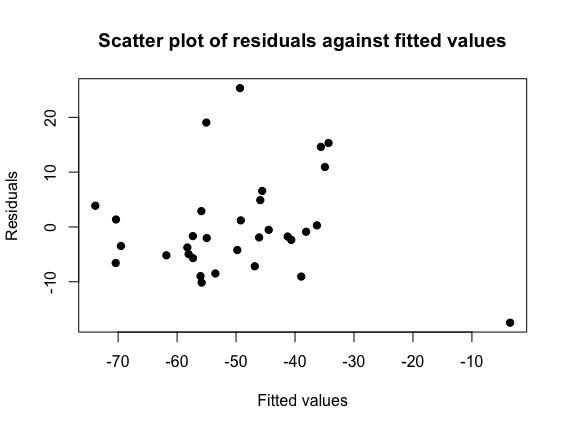
\includegraphics[width=0.75\linewidth]{scatterplot1}
			\caption{Residuals against $\hat{y}$}
			\label{scatterplot1}
		\end{figure}

		\begin{figure}[b]
			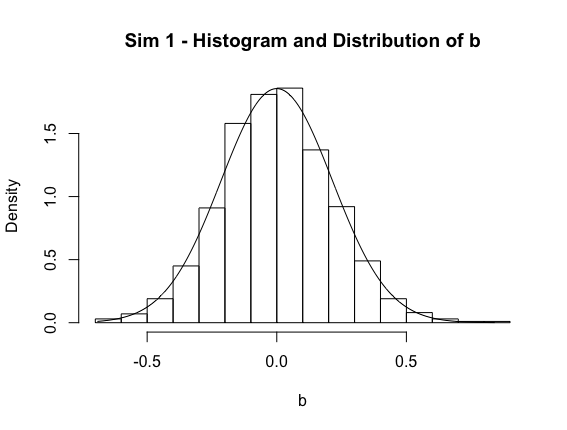
\includegraphics[width = 0.75\linewidth]{bhist}
			\caption{Histogram of $\hat{b}$, with theoretical distribution superimposed}
			\label{bhist}
		\end{figure}

		\begin{figure}[t]
			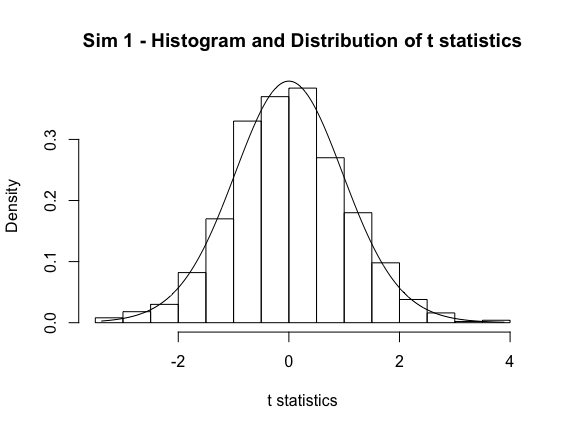
\includegraphics[width = 0.75\linewidth]{tstathist}
			\caption{Histogram of $t$, with theoretical distribution superimposed}
			\label{tstathist}
		\end{figure}

		\begin{figure}[b]
			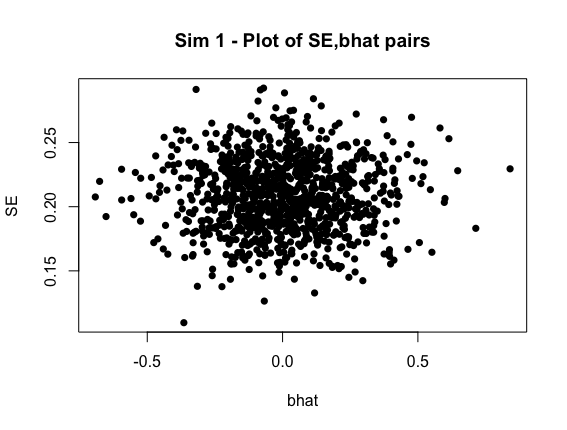
\includegraphics[width = 0.75\linewidth]{scatterplot2}
			\caption{Plot of $\left( \hat{b}, \hat{\sigma} \right)$.}
			\label{scatterplot2}
		\end{figure}

		\begin{figure}[t]
			\begin{tabular}{c|cccccccc}
				Sim & $\mu_{\hat{b}}$ & $\sigma_{\hat{b}}$ & $\mu_{\hat{b} | H_{0}}$ & $\sigma_{\hat{b} | H_{0}}$ & $\mu_{t}$ & $\sigma_{t}$ & $\mu_{\SE}$ & $\sigma_{\SE}$ \\
				\hline
				\hline
				Original & $-5.23\times 10^{-5}$ & 0.215 & 0 & 0.212 & $-6.46\times 10^{-4}$ & 1.057 & 0.209 & 0.0283 \\
				\hline
				Diff Param & $-0.00515$ & 0.354 & 0 & 0.353 & $-0.0106$ & 1.045 & 0.351 & 0.0468 \\
				\hline
				$H_{1}: b = 0.5$ & 0.4996 & 0.0143 & 0.5 & 0.212 & 36.228 & 4.969 & 0.014 & 0.0018 \\
				\hline
				New errors & $-0.00579$ & $0.204$ & 0 & 0.212 & $-0.00947$ & $0.996$ & 0.209 & 0.0389 \\
				\hline
			\end{tabular}
			\caption{Summary of Simulations}
			\label{simsum}
		\end{figure}
	% section figures (end)
\end{document}